\documentclass{fizraport}
\authorA{Krzysztof Stasiowski}
\authorB{Joanna Binek}
\team{2}{2a}{1}

\topic{Mostek Wheatstone'a }{32}{
Praktyczne zastosowanie praw Kirchhoffa i~sprawdzenie zależności określających opór zastępczy
dla połączeń szeregowych, równoległych oraz mieszanych.}
\carryOutDate{31.10.2018 r.}
\ftHandInDate{07.11.2018 r.}
\begin{document}
\maketitle

\section{Wstęp teoretyczny}
Na dołączonych przez nas~kartkach znajdują się~opracowane zagadnienia z~sekcji \mbox{,,zagadnienia kontrolne''} dla~tego doświadczenia, które odpowiadają wstępowi teoretycznemu.
\newline
\newline
Mostek Wheatstone’a jest układem do pomiaru (porównywania) oporów.Tworzy go
połączenie czterech oporów: $R_x$, $R_2$, $R_3$, $R_4$ oraz galwanometru o oporze $R_5$. Mostek jest zasilany z ogniwa galwanicznego lub zasilacza o sile elektromotorycznej $E$ i oporze wewnętrznym $R_E$ (\figref{fig:mostek})
\newpage %można pomyślec nad mniejszym marnotrawieniem papieru w~celu dołączenia naszych ręcznych zagadneń kontrolncyh
\addtocounter{page}{4}%żeby nasze kartki były zawarte w numeracji

\section{Układ pomiarowy}
 W~skład obwodu z~\figref{fig:mostek}] wchodzą:
\begin{enumerate}
    \item Listwa z~drutem oporowym, zaopatrzona w~podziałkę milimetrową i~kontakt ślizgowy,
umożliwiający zmiany długości odcinków $a$ i~$b$. 
    \item Opornica dekadowa $R_2$
    \item Symbolem $R_x$
 oznaczono zestaw oporników wmontowanych na~odpowiedniej płytce z~pleksiglasu.
    \item Mikroamperomierz G jako wskaźnik zerowania mostka Jego czułość można regulować. 
    \item Zasilacz stabilizowany 3A/30 V. 
\end{enumerate}

\begin{figure}[!htb]
	\centering
	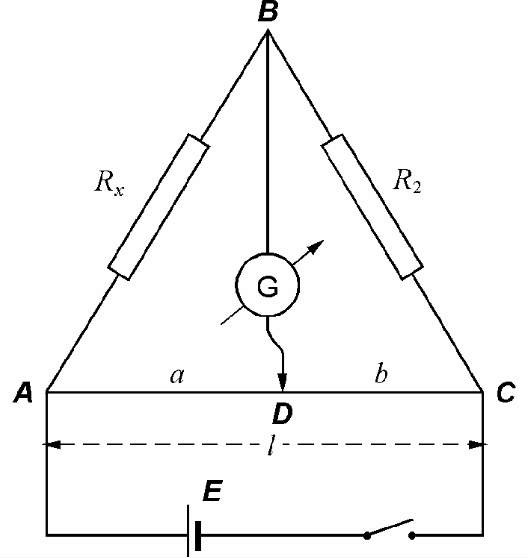
\includegraphics[scale=0.45]{4/mostek.png}
	\caption{ Schemat elektryczny mostka.}
	\label{fig:mostek}
\end{figure}


\section{Wykonanie ćwiczenia}
W~pierwszej kolejności połączyliśmy obwód elektryczny według schematu przedstawionego na~rysunku~(\figref{fig:mostek}) i~po sprawdzeniu
przez prowadzącego włączyliśmy zasilanie. Zmierzyliśmy długość drutu oporowego miarką o~niepewności pomiarowej ustalonej na~2mm.\\
Następnie wykonaliśmy 4 serie dziesięciu pomiarów, po~jednej dla~każdego nieznanego oporu wskazanego przez prowadzącego.

\bigskip
Analizowane kombinacje wskazane przez prowadzącego:
\begin{enumerate}
    \item $R_{x1}$
    \item $R_{x2}$
    \item $R_{x1}$, $R_{x2}$ równolegle
    \item $R_{x1}$, $R_{x2}$ szeregowo
\end{enumerate}
Wyniki pomiarów za~każdym razem zapisywaliśmy w~tabelach, które są~umieszczone w~sekcji \ref{sec:wyniki}.

\newpage% też te tabele z pomiarami
\addtocounter{page}{2}%żeby nasze kartki były zawarte w numeracji

\section{Wyniki pomiarów}
\vspace{-1.5em}
\label{sec:wyniki}
\begin{table}[!tbh]
\small
Długość drutu oporowego~=~\SI{1000}{\milli\metre}\\
W pierwszej serii pomiarów odrzucamy pomiary o~numerach 2,3 i~10.
\caption{Pomiar dla~połączenia przez opornik $R_{x1}$}
\centering
\begin{tabular}{|l|l|l|l|}
\hline
Nr pomiaru&Opór wzorcowy [\si{\ohm}] & a [\si{\milli\metre}] & $R_{x1}$ [\si{\ohm}]           \\ \hline
1&101.2              & 88     & 9.76    \\ \hline
2&50.3               & 250    & 16.77   \\ \hline
3&30.7               & 331    & 15.19   \\ \hline
4&20.0                 & 331    & 9.90    \\ \hline
5&11.0                 & 468    & 9.68    \\ \hline
6&7.5                & 559    & 9.51    \\ \hline
7&5.1                 & 653    & 9.60    \\ \hline
8&3.0                  & 751    & 9.05    \\ \hline
9&1.7                & 834    & 8.54    \\ \hline
10&0.2               & 659    & 0.39    \\ \hline
\end{tabular}
\end{table}
%
\begin{table}[!tbh]
\small
W drugiej serii pomiarów odrzucamy pomiary o~numerach 7 i~10.
\caption{Pomiar dla~połączenia przez opornik $R_{x2}$}
\centering
\begin{tabular}{|l|l|l|l|}
\hline
Nr pomiaru&Opór wzorcowy [\si{\ohm}] & a [\si{\milli\metre}] & $R_{x2}$ [\si{\ohm}]           \\ \hline
1&270.0                & 68     & 19.70 \\ \hline
2&112.0                & 151    & 19.92 \\ \hline
3&60.4               & 252    & 20.35 \\ \hline
4&37.2               & 350    & 20.03 \\ \hline
5&24.5               & 450    & 20.05 \\ \hline
6&16.4               & 551    & 20.13 \\ \hline
7&8.9                & 647    & 16.31 \\ \hline
8&6.0                  & 750    & 18.00 \\ \hline
9&3.3                & 847    & 18.27 \\ \hline
10&0.8               & 952    & 15.87 \\ \hline
\end{tabular}
\end{table}
%
\begin{table}[!tbh]
\small
W trzeciej serii pomiarów odrzucamy pomiary o~numerach 1,8 i~10.
\caption{Pomiar dla~połączenia równoległego oporników $R_{x1}$ i~$R_{x2}$}
\centering
\begin{tabular}{|l|l|l|l|}
\hline
Nr pomiaru&Opór wzorcowy [\si{\ohm}] & a [\si{\milli\metre}] & $R_{x3}$ [\si{\ohm}]           \\ \hline
1&180.0                & 56     & 10.678   \\ \hline
2&64.0                 & 150    & 11.294   \\ \hline
3&33.0                 & 252    & 11.118   \\ \hline
4&20.0                 & 355    & 11.008   \\ \hline
5&13.5               & 450    & 11.045   \\ \hline
6&9.4                & 549    & 11.443   \\ \hline
7&6.3                & 652    & 11.803   \\ \hline
8&4.7                & 733    & 12.903   \\ \hline
9&2.3                & 850    & 13.034   \\ \hline
10&1.0                 & 924    & 12.158   \\ \hline
\end{tabular}
%
\end{table}
\begin{table}[!tbh]
\small
W czwartej serii pomiarów odrzucamy pomiary o~numerach 1,2,4 i~10.
\caption{Pomiar dla~połączenia szeregowego oporników $R_{x1}$ i~$R_{x2}$}
\centering
\begin{tabular}{|l|l|l|l|}
\hline
Nr pomiaru&Opór wzorcowy [\si{\ohm}] & a [\si{\milli\metre}] & $R_{x4}$ [\si{\ohm}]           \\ \hline
1&540.0                & 51     & 29.02   \\ \hline
2&167.0                & 153    & 30.17   \\ \hline
3&91.0                 & 248    & 30.01   \\ \hline
4&54.0                 & 351    & 29.20   \\ \hline
5&37.0                 & 443    & 29.43   \\ \hline
6&24.3               & 550    & 29.70   \\ \hline
7&15.9               & 650    & 29.53   \\ \hline
8&10.0                 & 750    & 30.00   \\ \hline
9&5.2                & 851    & 29.70   \\ \hline
10&1.4               & 956    & 30.42   \\ \hline
\end{tabular}
\end{table}
\newpage

\section{Opracowanie wyników pomiarów:}
\subsection{Wyliczenie oporu oporników na~podstawie średniej:}
Wykorzystywany wzór:
\begin{align*}
   \overline{R} &= \frac{1}{n}  \sum\limits_{i=1}^{n}{R_{i}}
\end{align*}
\begin{enumerate}
    \item $R_{x_1}$:  \SI{9.43}{\ohm}
    \item $R_{x_2}$:  \SI{19.55}{\ohm}
    \item $R_{x_3}$:  \SI{11.410}{\ohm}
    \item $R_{x_4}$:  \SI{29.73}{\ohm}
\end{enumerate}

\subsection{Wyliczenie niepewności typu A dla~pomiaru oporu:}
Wykorzystywany wzór:
\begin{align*}
    u(R) &= \sqrt{\frac{1}{n\cdot(n-1)}\sum\limits_{i=1}^{n}{(R_{i} - \overline{R})^2}}  
\end{align*}
\begin{enumerate}
    \item $u(R_{x_1})$:  \SI{0.18}{\ohm}
    \item $u(R_{x_2})$:  \SI{0.32}{\ohm}
    \item $u(R_{x_3})$:  \SI{0.098}{\ohm}
    \item $u(R_{x_4})$:  \SI{0.17}{\ohm}
\end{enumerate}   

\subsection{Wyliczenie oporu zastępczego na~podstawie $R_{x_1}$ i~$R_{x_2}$ dla~połączenia równoległego oraz niepewności wyznaczenia:}
\begin{equation*}
    R_{{obl}} = \frac{R_{x1} \cdot R_{x2}}{R_{x1} + R_{x2}} = \SI{6.363}{\ohm}
\end{equation*}
\begin{equation*}
    u(R_{obl}) = \sqrt{\left [\frac{u(R_{x_1})\cdot R_{x_2}^2}{(R_{x_1} + R_{x_2})^2} \right ]  ^2 + \left [\frac{u(R_{x_2})\cdot R_{x_1}^2}{(R_{x_1} + R_{x_2})^2} \right] ^2} = \SI{0.087}{\ohm}%check if possible
\end{equation*}

\subsubsection{Porównanie wartości zamierzonej oporu zastępczego $R_{x_3}$ z~wartością obliczoną $R_{{obl}}$ w~granicach niepewności rozszerzonej $U(R_{x_3}-R_{{obl}})$ dla~$k=2$}
\begin{align*}
    |R_{x_3}-R_{{obl}}| &= \SI{5.05}{\ohm} \\
    U(R_{x_3}-R_{{obl}}) &= k\sqrt{[u(R_{x_3})]^2 + [u(R_{{obl}})]^2}  \\
    U(R_{x_3}-R_{{obl}}) &= \SI{0.27}{\ohm}
\end{align*}
Wyniki pomiaru nie~można uznać za~zgodne, ponieważ:
\begin{align*}
    |R_{x_3}-R_{obl}| > U(R_{x_3}-R_{obl}) 
\end{align*}    
\pagebreak


\subsection{Wyliczenie oporu zastępczego na~podstawie $R_{x_1}$ i~$R_{x_2}$ dla~połączenia szeregowego oraz niepewności wyznaczenia:}
\begin{equation*}
        R_{{obl}}= R_{x1} + R_{x2} = \SI{28.99}{\ohm}
\end{equation*}

\begin{equation*}
    u(R_{obl}) = \sqrt{u(R_{x_1})^2 + u(R_{x_2})^2} = \SI{0.37}{\ohm}
\end{equation*}

\subsubsection{Porównanie wartości zamierzonej oporu zastępczego $R_{x_4}$ z~wartością obliczoną $R_{{obl}}$ w~granicach niepewności rozszerzonej $U(R_{x_4}-R_{{obl}})$ dla~$k=2$}
\begin{align*}
    |R_{x_4}-R_{{obl}}| &= \SI{0.74}{\ohm} \\
    U(R_{x_4}-R_{{obl}}) &= k\sqrt{[u(R_{x_4})]^2 + [u(R_{{obl}})]^2}  \\
    U(R_{x_4}-R_{{obl}}) &= \SI{0.82}{\ohm}
\end{align*}
    
Wyniki pomiaru można uznać za~zgodne, ponieważ:
\begin{align*}
    |R_{x_4}-R_{obl}| < U(R_{x_4}-R_{obl}) 
\end{align*}

\section{Wnioski}
Zmierzone wartości oporu zastępczego są~w~granicach niepewności rozszerzonej zgodne z~wartościami obliczonymi dla~połączenia szeregowego, ale~nie~jest tak dla~połączenia równoległego.
Może być to wywołane z~następujących powodów:
\begin{enumerate}
    \item Kable użyte do~tego połączenia miały większą oporność, z~powodu zużycia,
    \item Przyłącza użyte do~równoległego połączenia, nie~zostały prawidłowo włożone,
    \item Biorąc pod uwagę fakt, że~wartości oporów, które~ wyznaczyliśmy dla~połączenia równoległego są~do~siebie bardzo podobne i~wszystkie są o~około \SI{5}{\ohm} większe od~teoretycznej wartości to~prawdopodobnie przyczyną nadwyżki o~\SI{5}{\ohm} jest sam~układ.
\end{enumerate}


\end{document}
